In this section, we introduce the timed automata modeling formalism, the UPPAAL modeling tool, and some relevant terminologies and concepts used throughout this paper.

% ===================================== Timed Automata ======================================
\subsection{Timed Automata}
\label{sub: timed_automata}
Timed automata is a hybrid mathematical modeling formalism in which a finite set of real-valued clocks are used to represent continuous time in a discrete-event system~\cite{alur1994_Theory_Timed_Automata}. Any real-time system whose behavior involves a predetermined set of actions can be represented as a network of timed automata. The system can be decomposed into its constituent components, and each component can be modeled as a timed automaton, which is a finite-state machine extended with clock variables~\cite{behrmann2004_Tutorial_UPPAAL}. A timed automaton is a tuple $(L, lo, C, A, E, I)$ where,
\par
$L$ is a set of locations
\par
$lo \in L$ is the initial location
\par
$C$ is the set of clocks 
\par
$A$ is a set of actions, co-actions, and the internal $\tau$-action
\par
$E \subseteq L \times A \times B(C) \times 2c \times L$ is a set of edges
\par
$I : L \to B(C)$ assigns invariants to locations 
\par
A timed automaton accepts timed words; infinite sequences in which each symbol is associated with a real-valued time of occurrence~\cite{alur1994_Theory_Timed_Automata}. At the simulation start, every single automaton in a network of timed automata begins with all of its clocks initialized to zero. The elapsed time is reflected in the change of clocks, representing the advance of time in reality. All clocks are independent of each other and can be reset at each transition to keep track of the elapsed time since the last reset. A transition may only be taken if the associated time constraint imposed upon that transition is satisfied by the current clock values. This feature allows us to model the timing properties of real-time systems and capture interesting qualitative and quantitative aspects such as periodicity, bounded response, and timing delays.

% ========================================== UPPAAL ===========================================
\subsection{Modeling in UPPAAL}
\label{sub: modeling_in_uppaal}
UPPAAL is an integrated tool environment that supports the modeling, validation, and verification of real-time systems as networks of timed automata~\cite{behrmann2004_Tutorial_UPPAAL}. The model can be extended with data types (e.g., bounded integers, arrays) while also allowing model checking for verification and validation of system properties. This academic endeavor, jointly developed by Uppsala University in Sweden and Aalborg University in Denmark, has received considerable research community support for research on timed automata in recent years. Our work uses the UPPAAL 4.1 development snapshot available under a free academic license\footnote{http://www.uppaal.org/}.
\par
% UPPAAL basic graphical notations figure
\begin{figure}[h!]
    \centering
    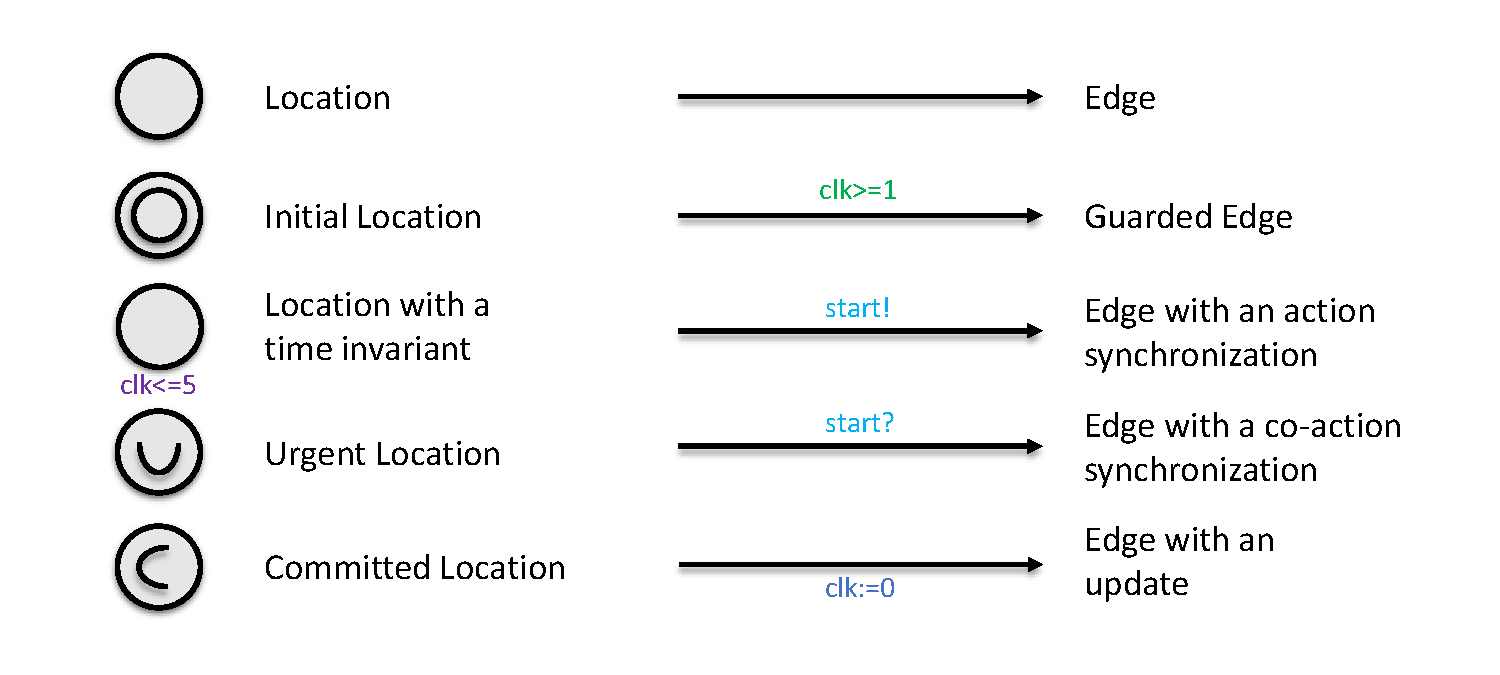
\includegraphics[width=\linewidth]{Figures/UPPAAL_Notations.pdf}
    \caption{UPPAAL graphical notations}
    \label{fig:uppaal_graphical_notations}
\end{figure}
\par
Figure~\ref{fig:uppaal_graphical_notations} shows some basic graphical notations used to model real-time systems in UPPAAL. Circles denote regular \notation{locations} that represent the state of an automaton performing a specific function. The \notation{initial location} (only one) of every automaton is depicted by an additional inner circle, specifying the starting behavior of that automaton when the system starts. Regular and \notation{initial locations} can be accompanied by a time invariant (depicted in violet text), which are time constraints imposed upon the location. A location with a time invariant must be left within the specified time constraint. Locations are also called \notation{states}, which is the term we will be using extensively throughout the paper.
\par
\notation{Urgent states}, denoted by an additional U inside the circle, represent states that are time-critical. These states cannot have any time invariants, and no time can pass while an automaton is in such a state. However, if any other automaton in the network is capable of performing an instantaneous action, that action is allowed. \notation{Committed states} (marked by an additional C) are even more restricted states that allow neither the passage of time nor any action by any other automaton unless that state is left.
\par
\notation{Edges}, depicted by arrows, represent the transition from one state to another. UPPAAL uses a handshaking mechanism to synchronize communication between different automata. During a transition, an \notation{edge} can send an action synchronization message (depicted in light blue text). This action message (\sync{start!}) must synchronize with another \notation{edge} with a corresponding co-action synchronization message (\sync{start?}), enabling the latter transition to take place.
\par
Individual automata can use state variables to record and share their state with other automata in the network. In addition, clock variables can be used to record the passage of time and impose timing constraints on locations and transitions. \notation{Guarded Edges} represent guarded transitions, where the transition is only allowed once the conditions (depicted in green text) imposed using state and/or clock variables on the transition, are satisfied. Additionally, edges can be accompanied by an \notation{update} command (depicted in blue text) that updates the value of a state and/or clock variable once the transition is completed.
\par